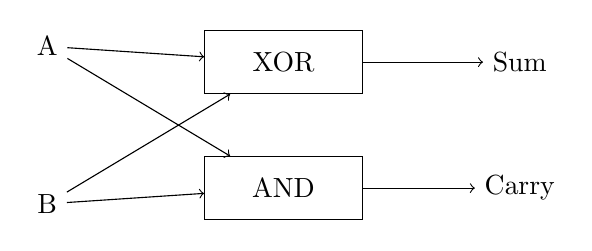
\begin{tikzpicture}[node distance=1.2cm]
\node (a) at (0,1) {A};
\node (b) at (0,-1) {B};
\node[draw,rectangle,minimum width=2cm,minimum height=0.8cm] (xor) at (3,0.8) {XOR};
\node[draw,rectangle,minimum width=2cm,minimum height=0.8cm] (and) at (3,-0.8) {AND};
\node (sum) at (6,0.8) {Sum};
\node (carry) at (6,-0.8) {Carry};
\draw[->] (a) -- (xor);
\draw[->] (b) -- (xor);
\draw[->] (a) -- (and);
\draw[->] (b) -- (and);
\draw[->] (xor) -- (sum);
\draw[->] (and) -- (carry);
\end{tikzpicture}
